\chapter{Refining the bounds}
\label{chap:bounds}

In previous chapters we have established that $\gdist(p)$ is asymptotically logarithmic, or, more precisely, that
\begin{align}
	2.73 \approx 3 \log_3(e) \leq \frac{\gdist(p)}{\log(p)} < 5 \log_2(e) \approx 7.21
\end{align}
for all primes $p$. The obvious question is -- what are the best possible constants in these estimates?

While the question is open, in this chapter we provide evidence which suggests that the following might be true:

\begin{conj}
\label{conj:lim-gdist}
Let $P$ be a real such that $P^3=P+1$. Then for primes $p$
\begin{align}
	\lim_{p \rightarrow \infty} \frac{\gdist(p)}{\log(p)} = 1/\log(P) \approx 3.56.
\end{align}
\end{conj}%

Our argument is based on the connection of $\gdist(p)$ to dissections of triangles. Recall that the key to establish the upper bound was the fact that $\gdist(p) \leq t(p)$. However, it seems that the following conjecture might be true:

\begin{conj}
\label{conj:gdistp-equals-tp}
Let $p$ be a prime. Then $\gdist(p) = t(p)$.
\end{conj}%

If that was the case, we would be able to establish bounds for $\gdist(n)$ by examining triangle dissections only. In particular, the following would imply Conjecture \ref{conj:lim-gdist}:

\begin{conj}
\label{conj:lim-hat-tn}
Let $P$ be a real such that $P^3=P+1$. Then
\begin{align}
	\lim_{n \rightarrow \infty} \frac{\hat t(n)}{\log(n)} = 1/\log(P).
\end{align}
\end{conj}%

The reason to consider triangle dissections is that we are able to generate them using a computer algorithm. Moreover, because it means no extra work for us, we consider prime dissections. By doing so we get the advantage that we do not have to restrict ourselves to prime sizes only.

In this chapter we present computational data of Rosendorf \cite{Rosendorf04} and of our own which support Conjecture \ref{conj:lim-hat-tn}. We begin by clarifying the role of constant $P$.


%%%
%%%
%%%
\section{Padovan sequence}

\begin{defn}
\emph{Padovan sequence} is a linear recurring sequence $(a_k)_{k \geq 1}$ defined by
\cosyalign{
	a_1 = a_2 = a_3 = 1, \quad a_{k+3} = a_{k+1}+a_k \ \ \mbox{ for } n \geq 1.
}%
The first few terms are $1, 1, 1, 2, 2, 3, 4, 5, 7, 9, 12, 16,\dots$
\end{defn}

For more information about the sequence see e.g. \cite{OEIS}.

Let $P, \lambda_1, \lambda_2$ be roots of the polynomial $x^3-x-1$, where $P$ is the only real root. Then we can write explicitly
\cosyalign{
	a_k = c_0P^k + c_1\lambda_1^k + c_2 \lambda_2^k
}%
for some complex constants $c_0,c_1,c_2$. Enumerating the values, we get $|\lambda_1|, |\lambda_2| < 1$ and $c_0 \approx 0.545$ is a real. Therefore $a_k \sim c_0P^k$, or $\log_P(a_k) \sim k$.

The number $P \approx 1.325$ is called \emph{the plastic constant}. As a side note, along with its mathematical properties, it has also its application in architecture \cite{Stewart96}.

\begin{defn}
Let $n$ be a positive integer. By $\spb(n)$ we denote an integer such that
\cosyalign{
	a_{\spb(n)-1} < n \leq a_{\spb(n)}.
}
\end{defn}

Note that $a_{\spb(n)}$ is the nearest term in Padovan sequence which is larger than or equal to $n$. Also $\spb(n) \sim \log_P(n)$.

\bigskip

Consider a trapezoid consisting of three unit triangles. In each step, we can attach a triangle to the longest side of the shape to get a pentagon. This way we get a spiral-like tiling. By adding two more triangles to the pentagon we obtain a $\circledast$-free dissection of a triangle. (Figures \ref{fig:spiral}, \ref{fig:spiral2}.)

\begin{figure}[htb]
\centering
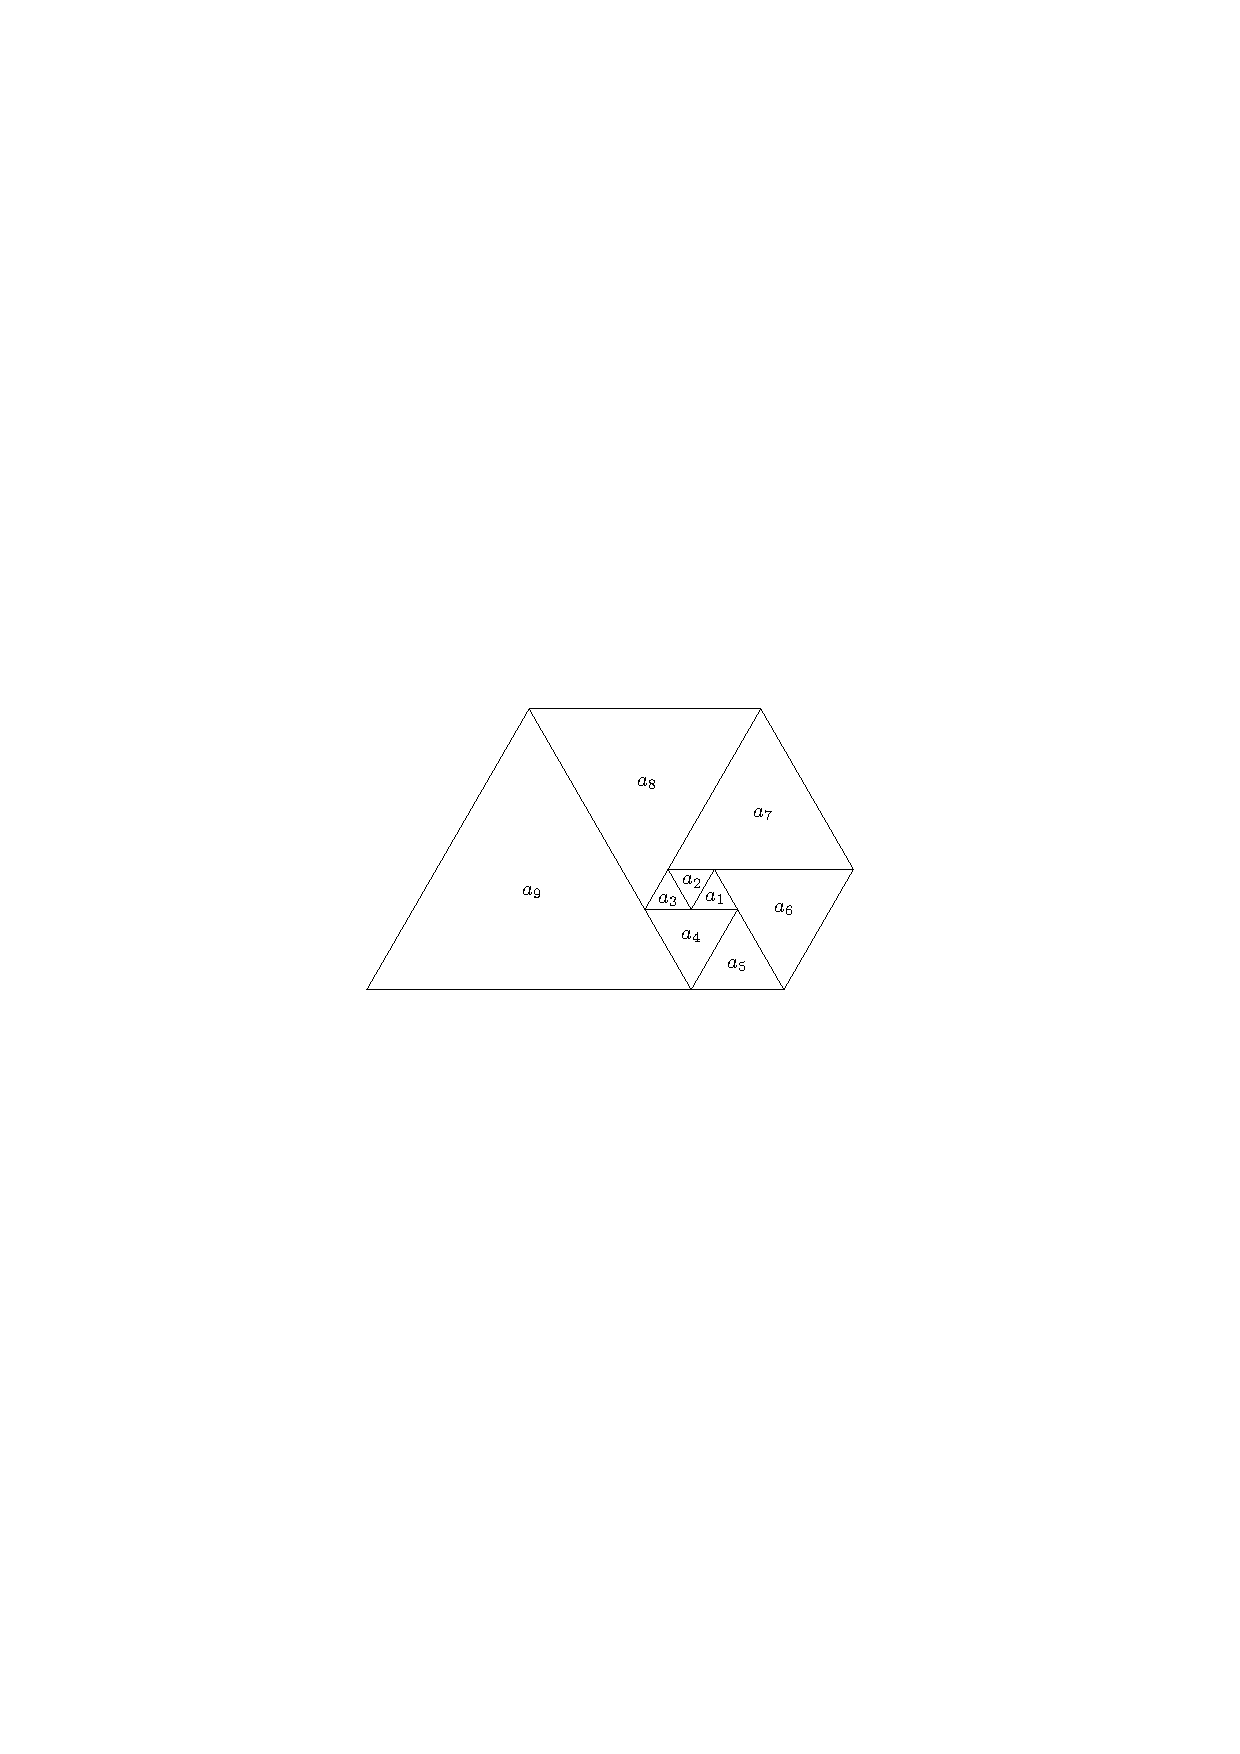
\includegraphics[width=0.6\textwidth]{img/spiral.pdf}
\caption{Spiral tiling.}
\label{fig:spiral}
\end{figure}

\begin{figure}[htb]
\centering
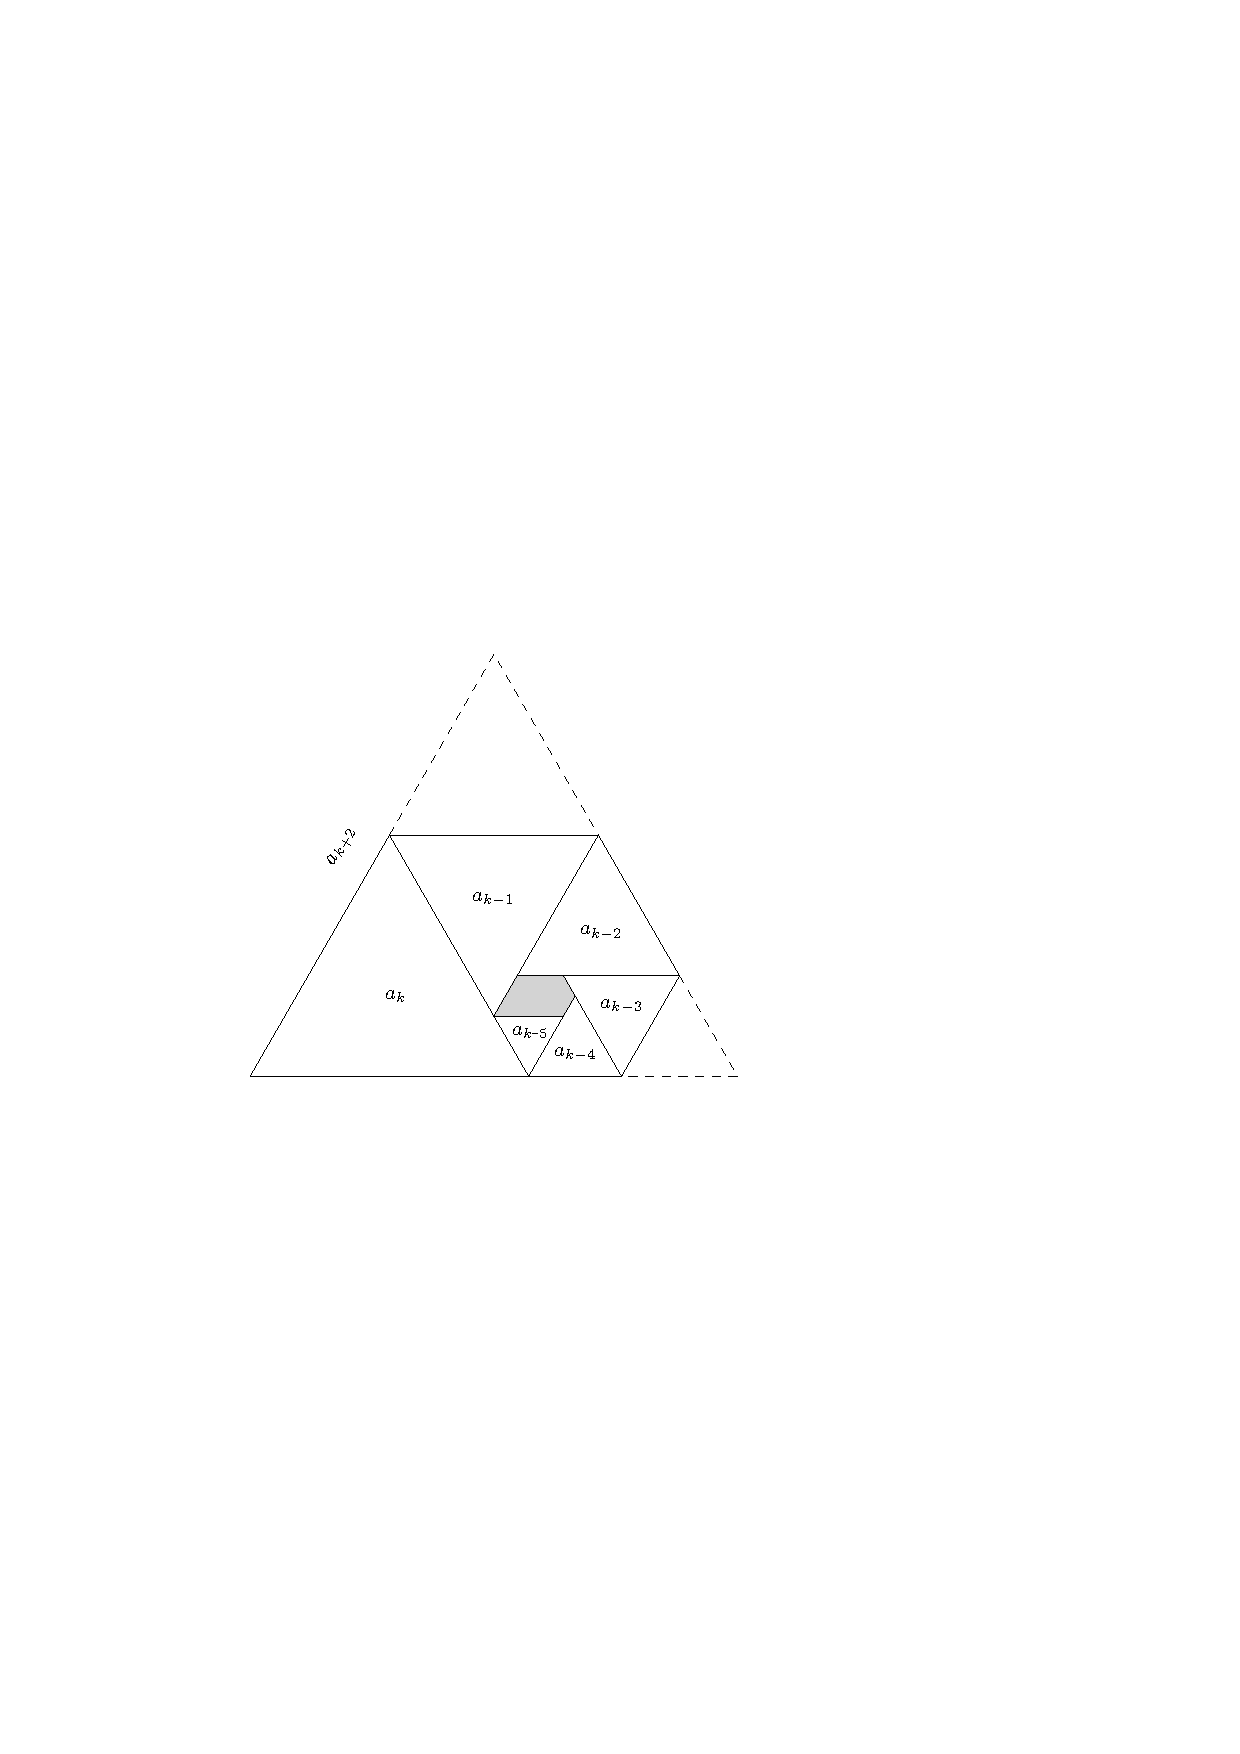
\includegraphics[width=0.6\textwidth]{img/spiral_triangle.pdf}
\caption{Completion of a pentagon into a triangle.}
\label{fig:spiral2}
\end{figure}

It is easy to derive that the sizes of the triangles are exactly the terms of Padovan sequence. Therefore we can construct a dissection of a triangle of side $a_{k+2}$ into $k+2$ triangles. Since in such a dissection there is always a triangle of side 1, we have
\cosyalign{
	\hat t(a_k) \leq k = \spb(a_k) \sim \log_P(a_k).\label{eq:tak-spbak}
}%

It would be desirable to generalize equation (\ref{eq:tak-spbak}) for all values on $n$. We conjecture that the following holds:
\begin{conj}
\label{conj:spbn}
$\spb(n)-1 \leq \hat t(n) \leq \spb(n)$.
\end{conj}%

\noindent
Because
\cosyalign{
	\frac{\spb(n)}{\log(n)} \sim \frac{\log_P(n)}{\log(n)} = 1/\log(P),
}%
this would imply Conjecture \ref{conj:lim-hat-tn}.

%%%
%%%
%%%
\section{Computational results of Rosendorf}
Based on Drápal's suggestion, Rosendorf studied in his master's thesis \cite{Rosendorf04} a modification of the spiral tiling, which can be applied to triangles of any size. Consider the following algorithm to dissect a triangle of size $n$:

\begin{alg} \ 
	\begin{cosyitemize}
		\item In the beginning, from two corners of the original triangle cut off two triangles to get a pentagon or a parallelogram;
		\item then, until the remaining shape is a triangle, cut off a triangle from the current shape to get either a pentagon, a parallelogram, a trapezoid or a triangle.
	\end{cosyitemize}
\end{alg}%

The algorithm is nondeterministic -- if the current shape is not a pentagon, we can choose the placement and the size of the triangle to be cut off. Rosendorf proved that these dissections are exactly those which are $\circledast$-free and do not contain a subset of triangles forming a proper convex hexagon. Following his notation, let us denote such a dissection as \emph{(M6)}, standing for ``missing hexagon''.

Rosendorf enumerated all minimal (M6) dissections of triangles of side less than 10252. The data show that
\begin{align}
	\hat{t}(n) \leq \spb(n)+2 \qquad\hbox{for $n < 10252$.}
\end{align}

On the other hand, he also proved that at least $\spb(p)$ triangles are needed in an (M6) dissection of a triangle of prime side $p$. That, however, is not true when we allow all $\circledast$-free dissections.


%%%
%%%
%%%
\section{Enumerations of minimal dissections}

We generated all triangle dissections up to size 23 and thus established values of $\hat t(n)$ for $n \leq 416$. For comparison, in \cite{DrapalHamalainen10} Drápal and Hämäläinen were able to generate dissections up to size 20, which corresponds to $n \leq 160$. They were, however, interested in other properties of triangulations, not in the values of $\hat t(n)$.

We use essentially the same algorithm as in \cite{DrapalHamalainen10}.\footnote{Although it is not absolutely clear from their paper, our implementation probably runs in better time complexity.} Separated connected spherical latin bitrades are equivalent to planar Eulerian triangulations (Theorem \ref{thm:connected-spherical-separated}), and planar Eulerian triangulations can be efficiently generated by Brinkmann and McKay's package \emph{plantri} \cite{BrinkmannMcKay99}. We will show an algorithm with which every triangle dissection can be reconstructed from a separated connected spherical latin bitrade.

\bigskip

Let $\D$ be a $\circledast$-free dissection of triangle $\Delta$ of side $n$, and $(T^*, T^\vartriangle)$ an embedding of it into the plane $x+y+z=0$.

\begin{lem}
$(T^*, T^\vartriangle)$ is a connected spherical latin bitrade.
\end{lem}
\begin{proof}
It suffices to show that the graph of $(T^*, T^\vartriangle)$ is connected and planar. A formal proof can be found e.g. in Tutte \cite{Tutte48}, we give only an illustration of it on Figure \ref{fig:triangulation-graph}. Black vertices correspond to elements of $T^*$, white to elements of $T^\vartriangle$.

\begin{figure}[htb]
\centering
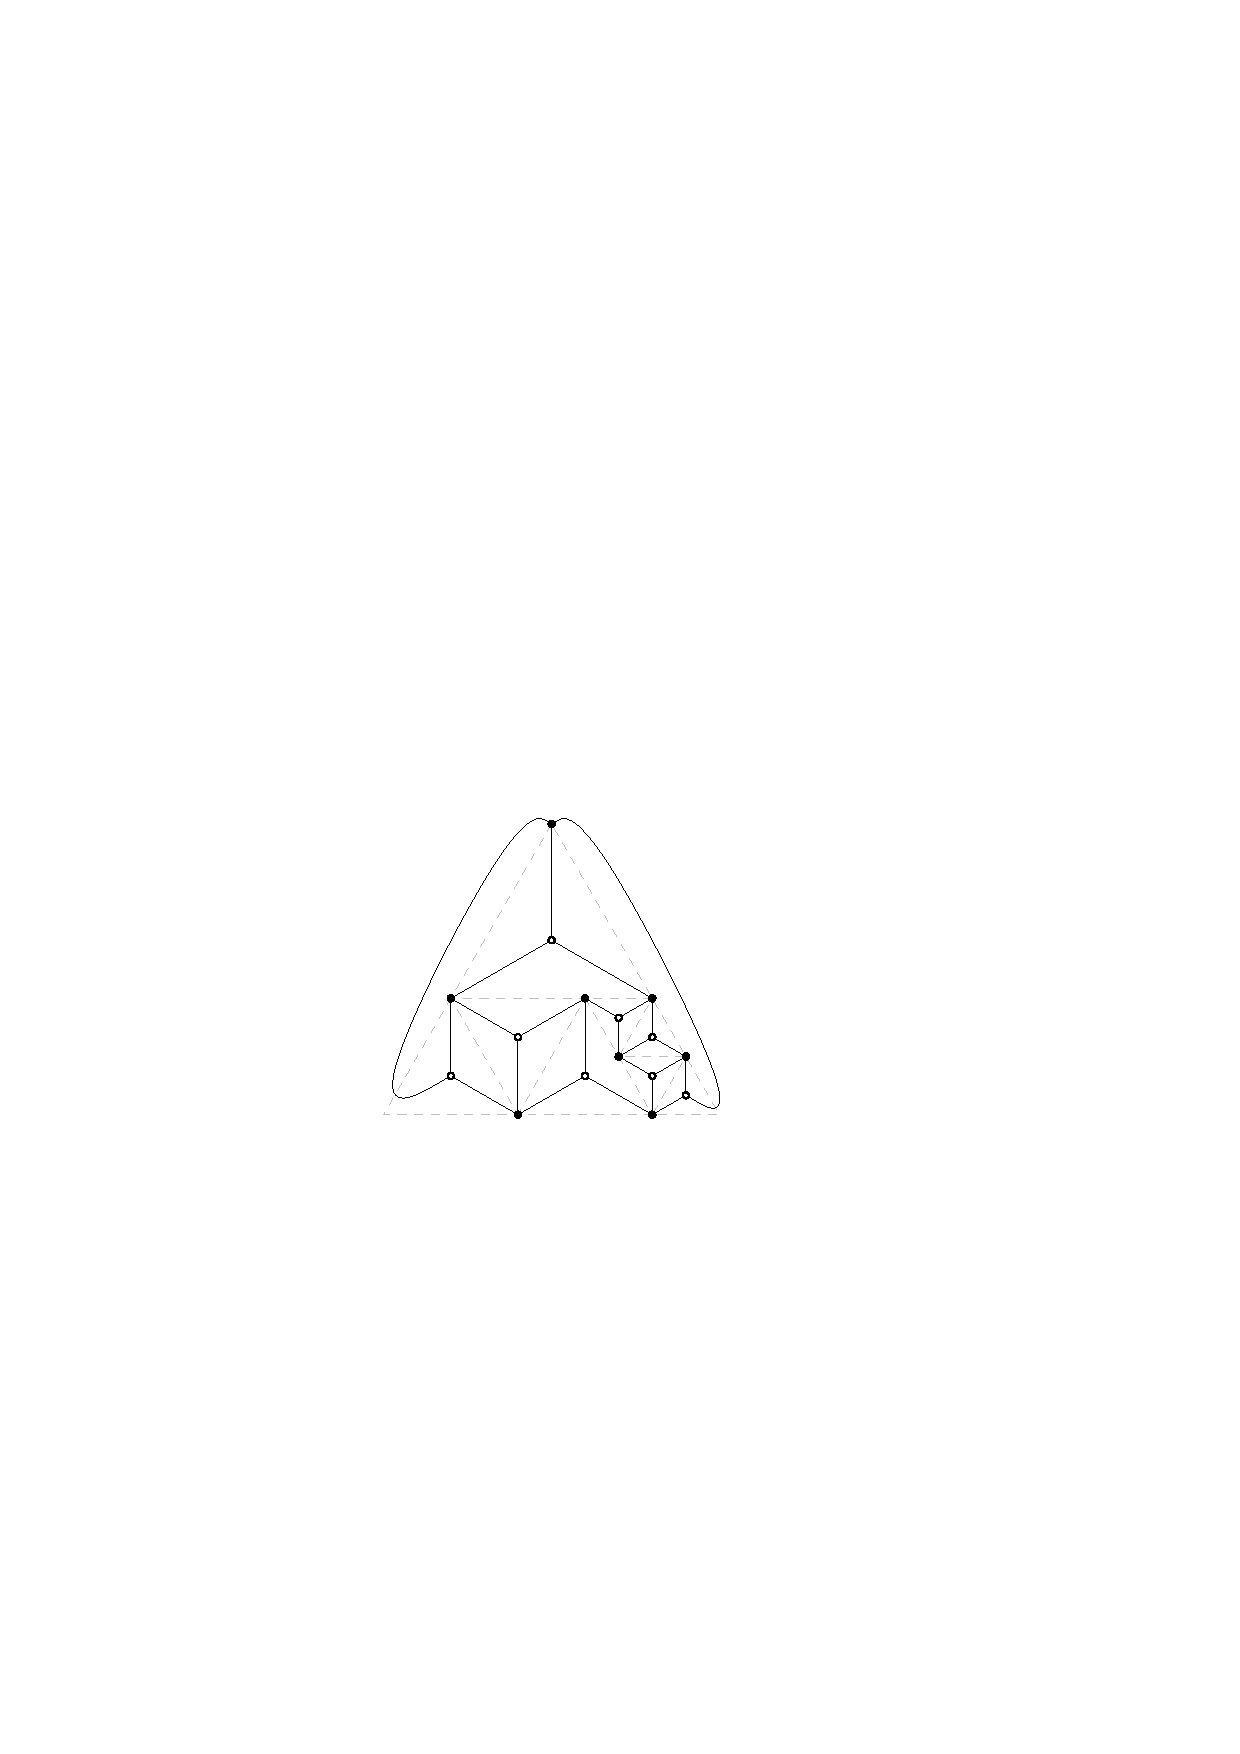
\includegraphics[width=0.5\textwidth]{img/triangulation_graph.pdf}
\caption{The graph obtained from a triangulation is connected and planar.}
\label{fig:triangulation-graph}
\end{figure}
\end{proof}

Let $(T,T')$ denote the separated latin bitrade obtained from $(T^*, T^\vartriangle)$ by the procedure described in Section \ref{sec:latin-bitrades}. Further denote $T$ and the support of $T$ such that:
\begin{itemize}
	\item $T = \{t_1, \dots, t_{|T|}\} \subset R \times C \times S$,
	\item $R = \{r_1,\dots,r_{|R|}\},\ 
		C = \{c_1,\dots,c_{|C|}\},\ 
		S = \{s_1,\dots,s_{|S|}\}$,
	\item $(r_1,c_1,s_1) \in T$,
	\item all elements of $X := R \cup C \cup S$ are used in $T$.
\end{itemize}%
From the construction of $(T,T')$, there is a natural homotopy $h:T \rightarrow T^*$ which projects $T$ onto $T^*$. Let us denote $h = (h_R, h_C, h_S)$. Since $T^* \subset \Z \times \Z \times \Z$, we have
\cosyalign{
	h_R: R \rightarrow \Z,\ h_C: C \rightarrow \Z,\ h_S: S \rightarrow \Z.
}%

Because embeddings of $\D$ are latin bitrades from the same main class (Lemma \ref{lem:embedding-bitrade-main-class}), $(T,T')$ does not depend on the choice of the embedding. Therefore let us adjust it a bit. Let $j \in [|T|]$ be such that $h(t_j) = (x,y,z) \in T^*$ represents the triangle $\Delta$. Then by rotation we can achieve $x + y + z = n$. Subsequently, by translation we can set $h_R(r_1) = h_C(c_1) = 0$.

Finally, denote by $M$ the matrix obtained from $M_T$ by excluding columns $r_1$ and $c_1$. Let us state a few lemmas in this context:

\begin{lem}
\label{lem:t-is-x-2}
$|T| = |X|-2$
\end{lem}
\begin{proof}
$(T, T')$ is a separated connected spherical latin bitrade. Its graph is planar with $2|T|$ vertices, $3|T|$ edges and $|X|$ faces (each face corresponds to one fixed coordinate). Plugging into Euler's formula yields the result.
\end{proof}

\begin{lem}
\label{lem:M-is-regular}
The matrix $M$ is regular.
\end{lem}
\begin{proof}
$M_T$ is of dimensions $|T|\times|X|$ and rank $|X|-2$ by Corollary \ref{cor:rank-mt}. The rest is clear by Lemma \ref{lem:t-is-x-2}.
\end{proof}

Recall that $T^*$ consists of vectors representing the vertices of triangles in the dissection $\D$ without the vertices of $\Delta$, but with the vector representing $\Delta$ included.

\begin{lem}
\label{lem:solution-n-0-0-0}
Denote by $e_i$ the unit vector with 1 on $i$-th coordinate, zeros elsewhere. Then the equation $Mv^T = ne_j^T$ has the only solution
\cosyalig{
	v = \big(\underbrace{h_R(r_2), \dots, h_R(r_{|R|})}_{|R|-1},\underbrace{h_C(c_2), \dots, h_C(c_{|C|})}_{|C|-1}, \underbrace{h_S(s_1), \dots, h_S(s_{|S|})}_{|S|}\big)
}%
\end{lem}
\begin{proof}
The vector $v$ is a solution directly from the construction of $T^*$. The uniqueness follows from Lemma \ref{lem:M-is-regular}.
\end{proof}

\begin{cor}
\label{cor:solution-1-0-0-0}
Continuing from Lemma \ref{lem:solution-n-0-0-0}, suppose $\D$ is a prime dissection. Then $h$ can be reconstructed from a vector $v$ such that
\cosyalign{
	Mv^T = e_j^T.
}%
\end{cor}
\begin{proof}
Define $f = (f_R, f_C, f_S)$ by
\cosyalig{
	n_0v = \big(\underbrace{f_R(r_2), \dots, f_R(r_{|R|})}_{|R|-1},\underbrace{f_C(c_2), \dots, f_C(c_{|C|})}_{|C|-1}, \underbrace{f_S(s_1), \dots, f_S(s_{|S|})}_{|S|}\big),
}%
where $n_0$ is the least common multiple of denominators of coordinates of $v$. Lemma \ref{lem:solution-n-0-0-0} implies that $n_0 \leq n$.

For contradiction, suppose $n/n_0 \ne 1$. Then either $n/n_0$ is an integer, in which case all coordinates in the embedding are multiples of $n/n_0$; otherwise they are multiples of the denominator of $n/n_0$. Either case contradicts the primality.

Therefore $n = n_0$ and $f=h$.
\end{proof}

\begin{lem}
Let $\D$ be a prime dissection. Then $h$ can be reconstructed from one of the columns of $M^{-1}$.
\end{lem}%
\begin{proof}
The $j$-th column of $M^{-1}$ is the unique solution to $Mv^T = e_j^T$. The rest is Corollary \ref{cor:solution-1-0-0-0}.
\end{proof}

The algorithm to generate all prime triangle dissections is as follows:

\begin{alg}\ 
\label{alg:tranquility}
\begin{cosyenumerate}
	\item Use \emph{plantri} to generate a planar Eulerian triangulation on $v$ vertices.
	\item Construct the corresponding separated connected spherical latin bitrade $(T,T')$. This is possible by Corollary \ref{cor:connected-spherical-separated}.
	\item Construct $M$, it is a matrix of size $(v-2) \times (v-2)$.
	\item Find $M^{-1}$. Every column describes a homotopy $h$ of $T$ into $\Z\times\Z\times\Z$.
	\item For each latin bitrade $(T^*,T^\vartriangle) := (h(T),h(T'))$ check that it is an embedding of a $\circledast$-free triangle dissection.
	\item Repeat for $(T',T)$.
\end{cosyenumerate}
\end{alg}%

Let us make a brief discussion about the algorithm. For a given graph its time complexity is $O(v^3)$, because the main part involves finding an inverse of a matrix.

We are also ought to mention how to perform step 5. $T^*$ contains coordinates of the points in the dissection (the special case with the triangle $\Delta$ is easily handled), and $T^\vartriangle$ defines which points to connect. Therefore a set of triangles can be constructed from $(T^*,T^\vartriangle)$.

We have to verify that the set is a valid $\circledast$-free dissection. A necessary condition is that all points in $T^*$ are distinct. Conveniently, under this condition the generated bitrades $(T^*,T^\vartriangle)$ were always separated.\footnote{To clarify, $\hat t(n)$ is realized by a latin bitrade corresponding to a triangle dissection of size $\hat t(n)$. The first such a bitrade that occured during execution of the algorithm was always separated. Therefore, there could possibly exist a bitrade which is not separated, yet of size $\hat t(n)$. However, the author believes, that the proof in \cite{DrapalHamalainenKala10} can be strengthened to show that if points in $T^*$ are distinct, then the dissection is always valid.} Drápal, Hämäläinen and Kala \cite{DrapalHamalainenKala10} proved that such bitrades yield valid $\circledast$-free triangulations.

\bigskip

The generated values of $\hat t(n)$ are listed in Appendix A. We were able to generate all dissections up to size $23$. By that we also established $\hat t(n) = 24$ for those $n$, for which at least one dissection into $24$ triangles was known. The data verify Conjecture \ref{conj:spbn} for $n \leq 416$.

In Appendix B we list minimal triangle dissections corresponding to values of $\hat t(n)$. Appendix C contains the implementation of the Algorithm \ref{alg:tranquility}.

As a final remark, note that
\cosyalign{
	t(n) = \min \{\hat t(d) \mid d \mbox{ divides } n\}.
}%
Therefore the values of $t(n)$ can be easily obtained from the generated values of $\hat t(n)$.


